\section{Business Procedures and Processes}

%%\subsection{Risk management process}



\subsection{Internal procedures}
The main internal procedure is the game creation. Besides this, as any other enterprise there are different internal procedures, human resources and IT maintenance, for example. The game creation follows the procedure shown in the figure \ref{fig:proc_game_creation} and is the following:

\begin{figure}[h] \centering
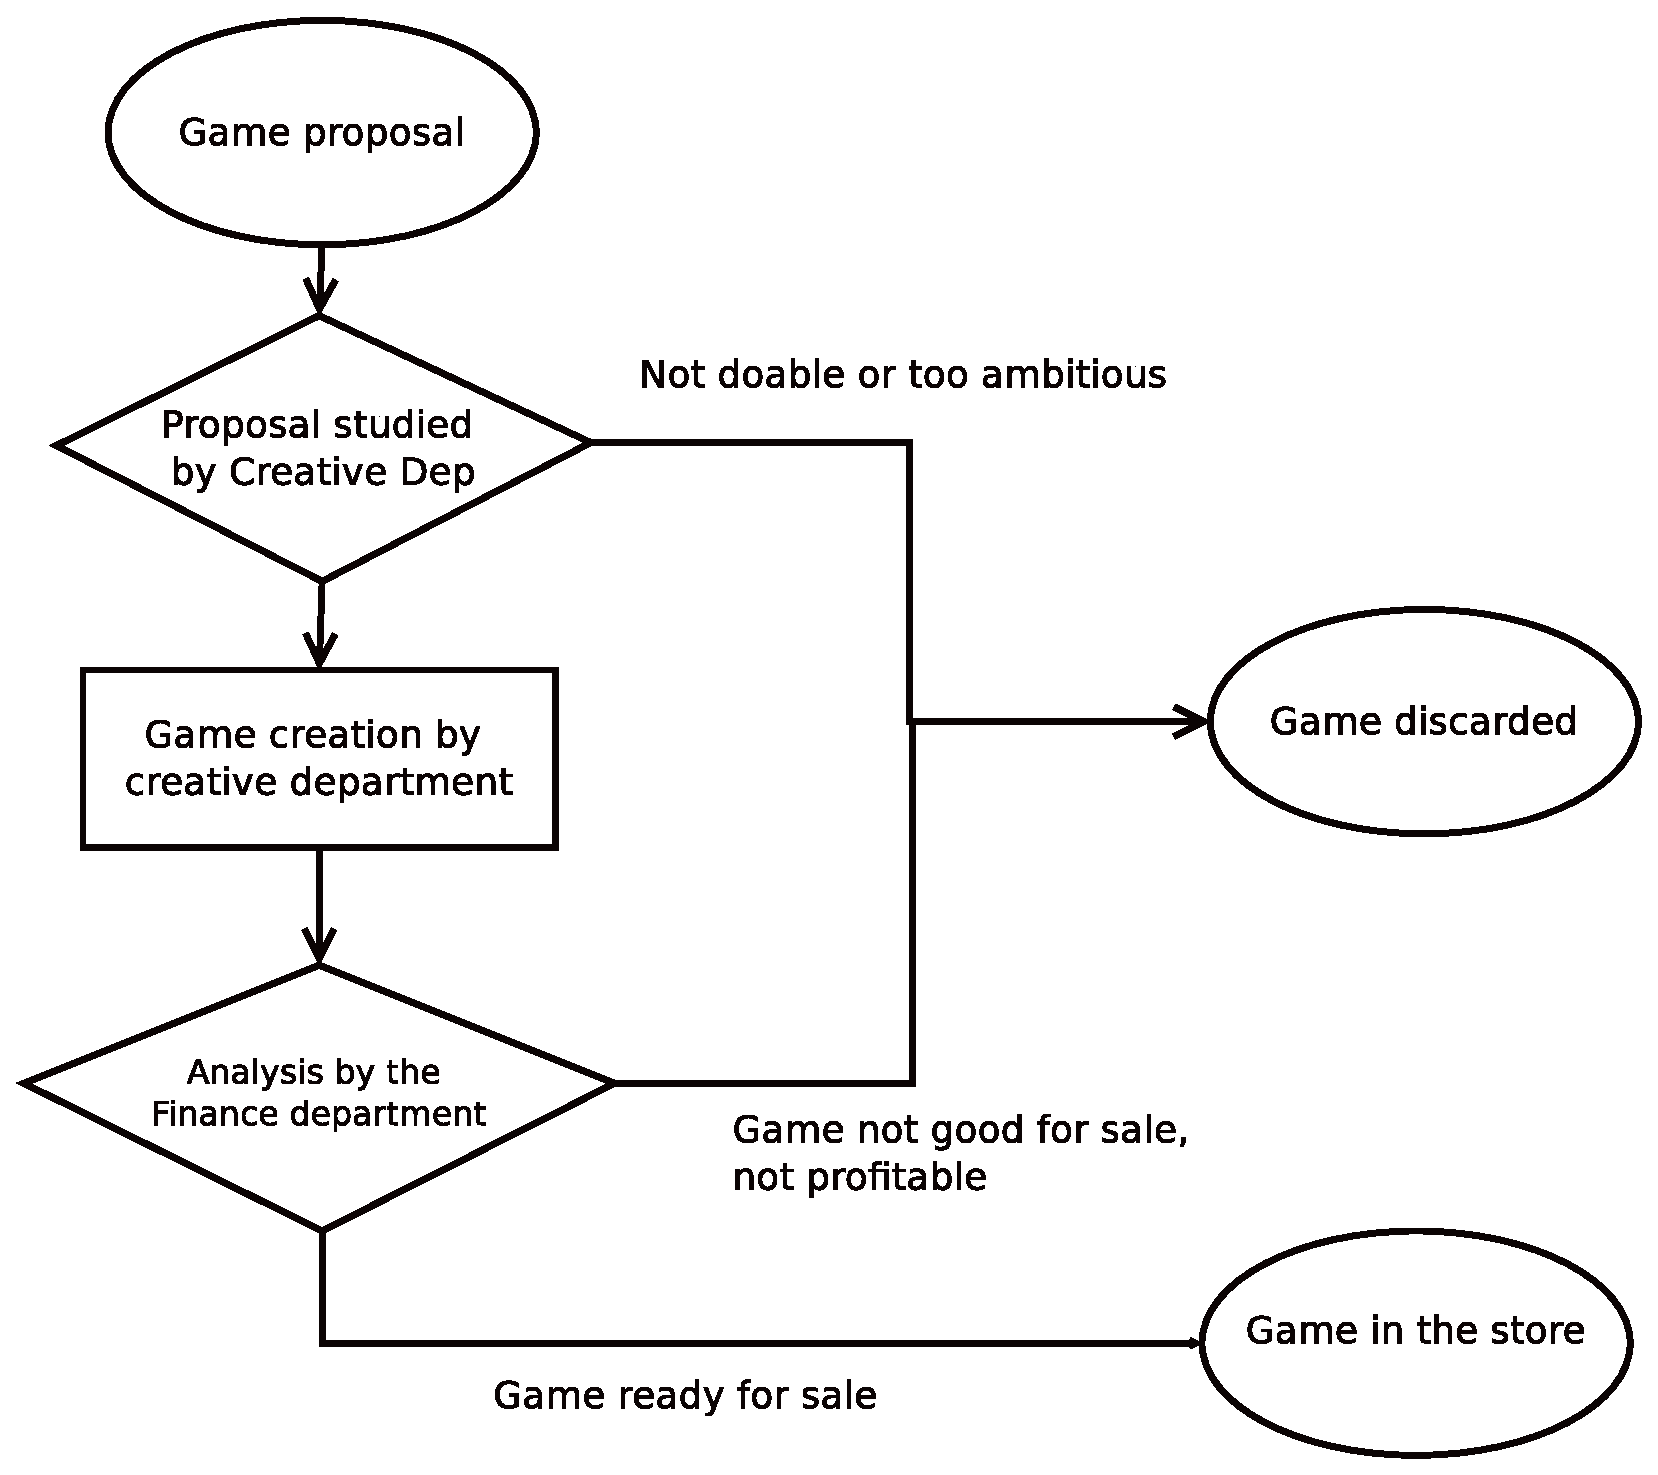
\includegraphics[width={0.7\textwidth}]{pictures/game_creation_process.eps}
\caption{Game creation process}
\label{fig:proc_game_creation}
\end{figure}

\begin {description}
\item{Idea creation: }This is the longer stage. It is a constant work in progress, during any stage the new ideas are taken in account. Once one project is finished a new idea is taken from the database.
\item{Idea study: }At this stage the idea is studied to check if it is doable, profitable and innovative. If it doesn't give the expected results the game idea is discarded.
\item{Game creation: }In this state the creative department starts the development of the project on itself. The development starts by programing the basic physics, story and the base program in general. When the 30\% of the estimated program is coded the design team starts working. At this early stage all the design is prepared for advertisement. While the game develops and the first alphas are launched the designers work more in the general graphics of the game.
\item{Game analysis: }When the game is around the 60\% through the development it's examined by the marketing department. If it gives clues for good and profitable sales it's approved and a marketing campaign is launched. If the game doesn't look good 	enough it's discarded.
\end {description}

\subsection{External procedures}
The main external procedure of Smoking games is the negotiation and signature of contracts with third party developers.

\begin{figure}[h]\centering
\includegraphics[ width={0.7\textwidth}]{pictures/third_party_game_process.eps}
\caption{Process for third party game distribution approval}
\label{fig:proc_third_party}
\end{figure}

This process as shown on the figure \ref{fig:proc_third_party} the process for signing a new contract is:

\begin{description}
\item{Project proposal reception: }The new game project is received in Smoking Games HQ.
\item{Project proposal analysis: }The project is given to the marketing department for market acceptance analysis and profit analysis. The marketing department will see the profitability of the project. In case the project doesn't give back a minimum the project will be discarded, and the developer told.
\item{Contract creation: }at this step the finance department will create a contract to present to the developer. The initial conditions of this contract have to have some flexibility for being able to negotiate. 
\item{Negotiation: }This newly created contract is presented and negotiated with the game developer. Depending on the result of this negotiation the project will be discarded or signed and validated.
\end{description}



An also important external procedure is the games sale through Smoke. This procedure is done using different payment options, credit card, pay pal or amazon payments, for example.